\section{MVC+S}

Jede Komponente der Anwendung unterliegt einer MVC-Struktur.
Komponenten beziehen sich hierbei auf Haupt-Features der App, wie etwa die Ordner-Ansicht oder Detail-Ansicht eines Dokuments.

Dabei sind die Abhängigkeiten aller Komponenten entsprechend des Dependency-Inversion-Prinzips umgekehrt. Jede View definiert sich ihren Controller selbst und erhält die Implementation über einen Riverpod Provider.

\subsection{Services}

Um den Zugriff auf die Datenbank zu vereinfachen wurde ein Persistenz-Service eingerichtet, sodass der Zugriff transparent geschieht.
Siehe Bild \ref{img:mvcps} für eine informelle Graphik der verwendeten Architektur.
Die Persistenz-Service ist modular, sodass Komponenten einfach ausgetauscht werden können.
Dies erreichen wir mithilfe des DAO-Pattern, um den tatsächlichen Zugriff auf den Speicher zu maskieren.
Im Sinne des Dependency-Inversion-Prinzips definiert der \verb|PersistenceService| die DAOs, die dieser benötigt.
Für mehr Information zum Aufbau der Persistenz-Schicht, siehe Kapitel \ref{chap:persistenz}.

Zusätzlich wird ein \verb|DbController| definiert, welcher dafür zuständig ist, die Datenbank zu laden und die DAOs zu instanziieren. Dessen Implementation - und damit die der DAOs - wird über Riverpod injected. Controller erhalten eine Instanz des \verb|PersistenceService| über einen Provider, welcher wiederum einen Provider für den DbController aufruft. Letzterer bestimmt die tatsächliche Implementation.

\begin{figure}[h]
  \centering
  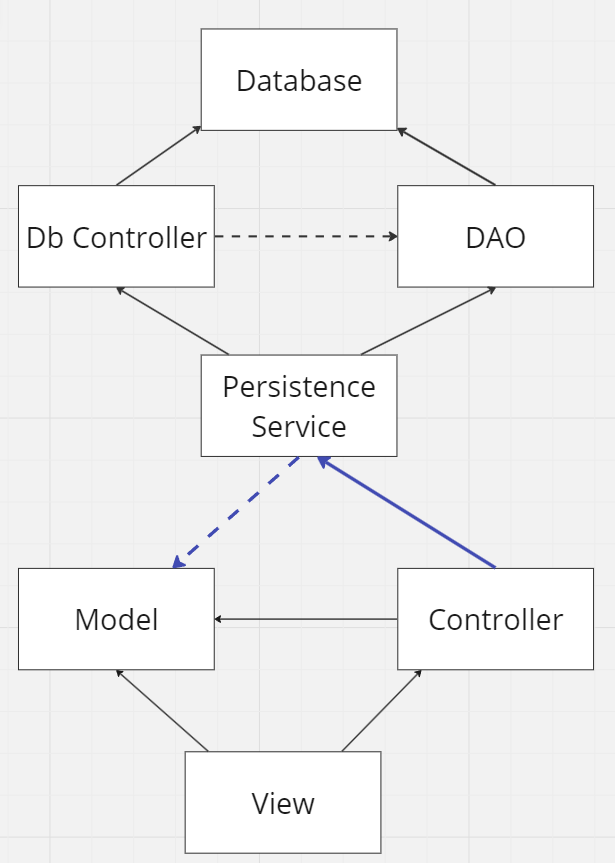
\includegraphics[height=0.5\textwidth]{figures/mvc_p_s.png}
  \caption{MVC+S Architektur}
  \label{img:mvcps}
\end{figure}

\section{Compositum Pattern für Ordner}

Die unterliegende Datenklasse für die Ordner-Struktur ist mittels des Compositum-Patterns umgesetzt.
Dazu wird die abstrakte Klasse \verb|FolderItem| genutzt, welche entweder ein \verb|SingleItem| oder ein \verb|Folder| ist, welcher weitere FolderItems enthält.
Dadurch können Ordner sehr leicht wiederum andere Ordner enthalten und die Unterscheidung dieser dennoch einfach.
So wird zum Besipiel in \verb|FolderItem| auch definiert, wie zur Detail-Ansicht dieser Entität navigiert werden kann, sodass sich die View nicht um diese Logik kümmern muss.

\section{State Management (Riverpod)}

Die App nutzt Riverpod zur Verwaltung des App-States. In einer Klasse sind die zahlreichen Provider als statische Variablen definiert, die von jeglichen Komponenten genutzt werden können.
Dabei gibt es für jede Komponente einen spezifischen Provider. Typischerweise ist das ein \verb|StateNotifierProvider| auf dem Model und dem Controller der Komponente oder die Async-Variante davon, wenn etwa Daten asynchron über den PersistenceService geladen werden müssen.

\subsection{Provider Families}

Die Provider für Ordner und Dokumente sind speziell, da diese eine ganze Reihe an Entitäten abdecken und nicht nur eine einzelne Instanz.
Dies lässt sich recht einfach über die Family-Provider von Riverpod lösen. Dabei muss beim Abruf des Provider ein Identifier \--- in diesem Fall die ID der Entität \--- übergeben werden und so erhält man einen neuen Provider für jede neue Entität.

Bei Dokumenten kommt noch dazu, dass diese über eine spezielle View editierbar sein sollen. Diese erlaubt, Änderungen zu puffern und bei Bedarf anzuwenden oder zu verwerfen.
Aus diesem Grund gibt es einen zweiten Family-Provider, welcher für das Editieren der Einträge verantwortlich ist.

Der Provider für Ordner ist so aufgebaut, dass bei Übergabe von null als Identifier der Provider für das Root-Verzeichnis des Profils zurückgeliefert wird.
Die \verb|Folder|-Klasse nutzt ein mixin '\verb|ExternalResource|', welches die Variablen \verb|isLoading| und \verb|hasError| definiert. Diese werden genutzt, wenn der Ordner asynchron geladen werden muss. Dadurch kann beim Aufruf von Unterordnern dieser eifnach aus den Inhalten des vorherigen gezogen werden und der View als initiale Daten übergeben werden, während die tatsächlichen Daten im Hintergrund neu geladen werden. Um diesen Aufruf zu vereinfachen wird eine selbst definierte Builder-Klasse genutzt; siehe Abschnitt \ref{sec:futures} zu angepassten \verb|FutureBuilder|n.

\section{Multi-Language Support}

Um Text in der App in verschiedenen Sprachen anzeigen zu können, wird eine abstrakte \verb|Language|-Klasse genutzt. Diese bietet Getter-Methoden für verschiedenste Strings, die von den Views benötigt werden.
Die Methoden-Namen sind so gewählt, dass das erste Element des Namens den Verwendungszeck und der Rest den Kontext angibt. So werden zum Beispiel Seiten-Titeln ein 'title' vorangestellt; konstanten Label-Texten ein 'lbl', Knöpfen ein 'btn', Textfeldern ein 'txt', Info-Benachrichtigugen ein 'info', Fehlerbenachrichtigungen ein 'err'.
Die Implementationen der Klasse bestimmen den genauen Text. Die korrekte Implementation erhält eine View wiederum durch den Riverpod-Provider für die App-Einstellungen.

\section{ErrorHandling}

Dadurch, dass die Views der App vorwiegend durch Slivers aufgebaut sind, können Overflow-Errors oder ähnliches in der Regel ausgeschlossen werden.
Die einzige ernstzunehmende Fehlerquelle der App ist die Persistenz-Schicht. Dabei wird allerdings selten eine tatsächliche Exception geworfen, sondern einfach \verb|null| zurückgeliefert. Aus diesem Grund werden die meisten Daten mittels Methoden zur Null-Safety verwendet. So liefert zum Beispiel der Provider für Dokumente ein \verb|SingleItem?| und die \verb|contents| der \verb|Folder|-Klasse sind eine \verb|List<FolderItem>?|.

\subsection{Angepasste FutureBuilders} \label{sec:futures}

Um mit all diesen verschiedenen Zuständen und zusätzlich noch der Asynchronität umgehen zu können werden eigens geschriebene Varianten des \verb|FutureBuilder|-Widgets verwendet.
Diese kommen in 3 Varienten: einmal für die Standard \verb|Future|s von Dart, dann für die \verb|AsyncValue|s von Riverpod und letztlich für unsere eigenen \verb|ExternalResource|s.
Diese Builder werden dann mit dem entsprechenden asynchronen Wert und einer Methode initialisiert, die das Widget bei erfolgreichem Laden baut. Im Fall eines Fehlers oder wenn null zurückgeliefert wird, wird stattdessen ein entsprechendes \verb|ErrorMessage|-Widget zurückgeliefert oder auch eine \verb|InfoMessage| für die spezifischen ListBuilder-Varianten, falls die Liste leer ist.
